\documentclass[aspectratio=169]{beamer}

\usetheme{Madrid}
\usecolortheme{default}
\usefonttheme{professionalfonts}
\setbeamertemplate{navigation symbols}{}
\setbeamertemplate{caption}[numbered]

\usepackage[utf8]{inputenc}
\usepackage[T1]{fontenc}
\usepackage{lmodern}
\usepackage{booktabs}
\usepackage{array}
\usepackage{graphicx}
\usepackage{tikz}
\usepackage{pgfplots}
\pgfplotsset{compat=1.18}
\usepackage{hyperref}
\usepackage{xcolor}

\definecolor{DeepBlue}{RGB}{20,55,90}
\definecolor{Accent}{RGB}{0,115,153}
\definecolor{SoftGray}{RGB}{245,247,250}

\setbeamercolor{title}{fg=DeepBlue}
\setbeamercolor{frametitle}{fg=DeepBlue}
\setbeamercolor{structure}{fg=Accent}
\setbeamercolor{block title}{bg=Accent!15,fg=DeepBlue}
\setbeamercolor{block body}{bg=SoftGray,fg=black}
\setbeamertemplate{footline}{\hfill\insertframenumber{}/\inserttotalframenumber\hspace{1em}\vspace{0.5em}}

\title[AI for Biomedical \& Critical Systems]{AI for Biomedical Systems \& Critical Systems}
\subtitle{Safety, reliability, regulation, and deployment patterns}
\author{Kelly Powell}
\institute{UAB Heersink School of Medicine}
\date{June 2026}

\begin{document}

\begin{frame}[plain]
\titlepage
\end{frame}

\begin{frame}{Why this topic matters}
AI is transforming biomedical engineering --- from imaging and diagnostics to wearables, prosthetics, and personalized treatment planning. In critical systems, the same capabilities create higher stakes: errors can affect patient safety, infrastructure, or essential services.
\begin{itemize}
  \item Biomedical AI must be accurate, explainable, and clinically useful.
  \item Critical AI must also be robust, monitored, and governable.
  \item The best systems combine performance with safety engineering.
\end{itemize}
\end{frame}

\begin{frame}{Biomedical AI applications}
\begin{columns}[T,onlytextwidth]
  \column{0.5\textwidth}
  \begin{block}{Core use cases}
    \begin{itemize}
      \item Medical imaging and computer-aided diagnosis.
      \item Predictive analytics for patient deterioration.
      \item Personalized medicine and treatment optimization.
      \item Smart devices, wearables, and prosthetics.
    \end{itemize}
  \end{block}
  \column{0.5\textwidth}
  \begin{block}{Value created}
    \begin{itemize}
      \item Faster detection and triage.
      \item Better use of complex multi-modal data.
      \item More adaptive care pathways.
      \item Continuous monitoring outside the clinic.
    \end{itemize}
  \end{block}
\end{columns}
\end{frame}

\begin{frame}{What makes a system critical}
A system is critical when failures can cause serious harm --- especially to health, rights, or essential services. That changes the engineering bar from ``works well'' to ``works reliably under uncertainty.''
\begin{itemize}
  \item \textbf{Safety impact:} harm to patients or operators.
  \item \textbf{Operational impact:} outages, delays, or cascading failures.
  \item \textbf{Decision impact:} automated recommendations in high-stakes settings.
  \item \textbf{Governance impact:} auditability, accountability, and oversight.
\end{itemize}
\end{frame}

\begin{frame}{Risk lifecycle}
\begin{block}{A practical AI lifecycle for critical deployments}
  \begin{enumerate}
    \item Define intended use, boundaries, and failure modes.
    \item Validate data quality, representativeness, and provenance.
    \item Test performance across subgroups and edge cases.
    \item Deploy with human oversight, monitoring, and rollback paths.
    \item Reassess drift, incidents, and post-market performance.
  \end{enumerate}
\end{block}
\end{frame}

\begin{frame}{Safety and reliability controls}
\begin{columns}[T,onlytextwidth]
  \column{0.5\textwidth}
  \begin{block}{Technical controls}
    \begin{itemize}
      \item Redundancy and failover.
      \item Input/output validation.
      \item Robustness and adversarial testing.
      \item Continuous monitoring for drift and anomalies.
    \end{itemize}
  \end{block}
  \column{0.5\textwidth}
  \begin{block}{Operational controls}
    \begin{itemize}
      \item Human-in-the-loop review for high-impact decisions.
      \item Clear escalation and incident response.
      \item Versioning and rollback capability.
      \item Periodic audits and documentation updates.
    \end{itemize}
  \end{block}
\end{columns}
\end{frame}

\begin{frame}{Governance framework: NIST AI RMF}
The NIST AI Risk Management Framework organizes trustworthy AI work into four connected functions. It treats AI risk as an ongoing program rather than a one-time review.
\begin{table}
  \centering
  \begin{tabular}{p{2.4cm}p{7.2cm}}
    \toprule
    \textbf{Function} & \textbf{Purpose in critical biomedical AI} \\
    \midrule
    Govern  & Assign accountability, policy, and oversight. \\
    Map     & Identify context, stakeholders, and harms. \\
    Measure & Evaluate model performance, bias, and robustness. \\
    Manage  & Mitigate risks, monitor operations, and respond to incidents. \\
    \bottomrule
  \end{tabular}
\end{table}
\end{frame}

\begin{frame}{Deployment architecture}
\begin{center}
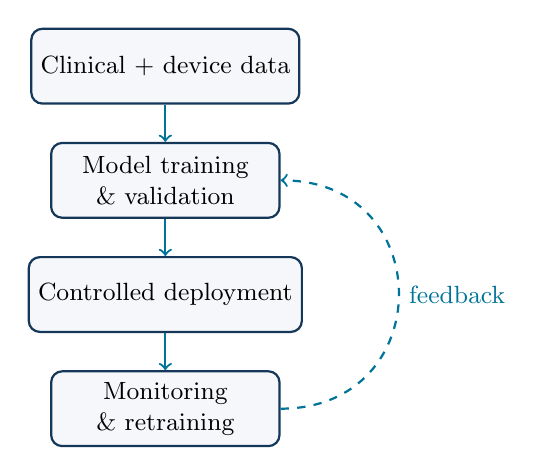
\begin{tikzpicture}[node distance=1.45cm, every node/.style={font=\small}]
  \tikzstyle{box}=[draw=DeepBlue, rounded corners, thick, fill=SoftGray,
                   align=center, minimum width=2.9cm, minimum height=0.95cm]
  \node[box] (data)    {Clinical + device data};
  \node[box, below of=data]    (model)   {Model training \\ \& validation};
  \node[box, below of=model]   (deploy)  {Controlled deployment};
  \node[box, below of=deploy]  (monitor) {Monitoring \\ \& retraining};
  \draw[->, thick, color=Accent] (data)    -- (model);
  \draw[->, thick, color=Accent] (model)   -- (deploy);
  \draw[->, thick, color=Accent] (deploy)  -- (monitor);
  \draw[->, thick, dashed, color=Accent]
    (monitor.east) .. controls +(2,0) and +(2,0) ..
    node[right]{feedback} (model.east);
\end{tikzpicture}
\end{center}
\end{frame}

\begin{frame}{Research and practice agenda}
\begin{itemize}
  \item Build domain-specific benchmarks for biomedical reliability and safety.
  \item Combine model metrics with system-level metrics like latency and downtime.
  \item Study human-AI collaboration in clinical workflows.
  \item Treat cybersecurity, privacy, and safety as shared design requirements.
  \item Use post-deployment monitoring to close the loop from research to care.
\end{itemize}
\end{frame}

\begin{frame}{Closing message}
AI in biomedical systems is most valuable when it improves outcomes without introducing unacceptable risk. In critical systems, success depends on pairing machine learning with engineering discipline, governance, and continuous oversight.
\vspace{0.5em}
\begin{block}{Takeaway}
  High-performing AI is not enough; critical biomedical AI must also be safe, traceable, and resilient.
\end{block}
\end{frame}

\begin{frame}[allowframebreaks]{Selected references}
\footnotesize
\begin{thebibliography}{9}
  \bibitem{beamer}  UMass Library, \emph{LaTeX: Beamer (Presentations)}, 2024.
  \bibitem{slides}  A.~N. Bahkali et al., \emph{Ten simple rules for effective presentation slides}, 2021.
  \bibitem{nist}    NIST, \emph{AI Risk Management Framework (AI RMF 1.0)}, 2023.
  \bibitem{biomed}  Public reviews and overviews on AI in biomedical engineering and biomedical sciences.
\end{thebibliography}
\end{frame}

\end{document}
